\section{Laboratory work implementation}

\subsection{Tasks and Points}

\begin{quote}
\begin{description}

	\item Basic Level (nota 5 - 6) :
	
	initializeaza un nou repositoriu \\
	configureaza-ti VCS\\
	crearea branch-urilor (creeaza cel putin 2 branches)\\
	commit pe ambele branch-uri (cel putin 1 commit per branch)

	\item Normal Level (nota 7 - 8):
	
	seteaza un branch to track a remote origin pe care vei putea sa faci push\\
	reseteaza un branch la commit-ul anterior\\
	salvarea temporara a schimbarilor care nu se vor face commit imediat\\
	folosirea fisierului .gitignore
	
	\item Advanced Level (nota 9 - 10):
	
	merge 2 branches\\
	rezolvarea conflictelor a 2 branches\\
	comezile git care trebuie cunoscute
	\item Bonus Point (+1):\\
	Folosirea tag-urilor pentru marcarea schimbarilor simnificative precum release-ul.

\end{description}
\end{quote}

\subsection{Analiza lucrarii de laborator}

Inainte de a incepe indeplinirea sarcinelor au fost efectuati citiva pasi aditionali, ce tin de pregatirea calculatorului pentru a putea utiliza acest sistem de versionare a codului. Am ales un sistem descentralizat deoarece acesta ne ofera posibilitati mai ample, referitor la controlul distribuit al versiunelor, gestionarea si revizuirea codului cit si vizualizarea activitatii proectului fata de sistemul centralizat. In special acesta fiind un model de source control ce permite partajarea surselor in mod distribuit intre membrii echipelor fara a depinde de un repozitoriu central.

\begin{flushleft} %
	\text{\itshape Instalarea si setarea sistemului Git sa efectuat conform manualului oferit de situl oficial git-scm.com.} 
\end{flushleft}

Utilizind serviciile prestate de reteaua sociala (GitHub) pentru proiecte cu versionarea bazata pe Git, am creat un cont pe \emph{\url{www.github.com}} care detine repozitoriul laboratorului efectuat.

\newcommand*{\authorimg}[1]{%
	\raisebox{-.3\baselineskip}{%
		\includegraphics[
		scale = 0.5, % or use height and width
		%height=\baselineskip,
		%width=\baselineskip,
		keepaspectratio,
		]{#1}%
	}%
}
\begin{itemize}
	\item[\authorimg{img/1.png}]
	\begin{center}
		Link la repozitoriu: \url{https://github.com/CristianGodonoaga/MIDPS}
	\end{center}
\end{itemize}

%\includegraphics[scale = 0.5]{img/img_name.png}

Pentru a asigura o comunicare securizata a datelor intre doua statii am utilizat protocolul de retea SSH. Acesta se foloseste de criptarea cu \emph{\textbf{\href{https://en.wikipedia.org/wiki/Public-key_cryptography}{chei asimetrice}}} ce furnizeaza un mod mai sigur de logare (comunicare) intr-un server cu SSH decit folosind o parola obisnuita. La generarea acestor perechi de key se utilizeaza un mecanizm special care ne ofera doua siruri lungi de caractere: o cheie publica si o cheie privata.

Intrun prim pas se creaza perechea de chei pe masina client:
\begin{quote}\tt
	\$ssh-keygen -t rsa \hfill (Fig.~\ref{fig:generarea_ssh_key})
\end{quote}

%\begin{description}
%	\item[-t rsa] tipul de cheii generate
%\end{description}

Dupa ce am introdus comanda de generare a cheii am primit citeva intrebari ce tine de marirea securitatii prin protejarea cheii privade, cu o parola de acces. Odata ce perechea de chei este generata plasam cheia publica pe serverul GitHub (Fig.~\ref{fig:add_key_onserver}).

Pentru a incepe utilizarea sistemului Git, mai intii este nevoie de setarea configuratiei de baza. Aceste configurari pot fi facute in trei modalitati, ele vor determina cit de amplu va fi aplicarea acestora.
Utilizind comenzile:
\begin{quote}\tt
	\$git config --global user.name "Godonoaga C."\\
	\$git config --global user.email "some@email.com" \hfill(Fig.~\ref{fig:generarea_ssh_key})
\end{quote}
%\begin{description}
%	\item[\tt\$git config --system] \hfil Configurare la nivel de sistem. 
%	\item[\tt\$git config --global] \hfil Configurare la nivel de utilizator.
%	\item[\tt\$git config --local] \hfil Configurare la nivel de proiect (by default).
%	\item[\tt\$git config --file <filename>] \hfil Configurare din fisierul concret
%\end{description}
am setat numele si posta la nivel de utilizator, ce ne permite utilizarea acestor date in viitor pentru oarecare alt proiect al acestuia fara a le specifica in parte.
Deoarece aceste setari depind foarte mult de necesitatea utilizatorului nu exista o varianta exacta ce tine de setarea sistemului Git.

Pentru a da start sistemului si anume pentru a monitoriza schimbarile in proiectul necesar se utilizeaza comanda {\tt \$git init}, aceasta va insemna ca noi avem nevoie de monitorizarea schimbarilor a tuturor fisierilor ce se afla in folderul curenta (creareaza un repository).




Explica fiecare din task-urile realizate. Explica acesta cu cuvintele tale. Cu cit mai bine va fi explicat, 
\textbf{git command --example "test"}
cu atit mai putine intrebari vei avea la aparare.

\begin{lstlisting}
git config --global user.name ""
\end{lstlisting}

\newcommand{\code}[1]{\texttt{#1}}
\code{git configss}
\tt git code



\subsection{Imagini}

\begin{figure}[htb]
	\begin{center}
		\centering
		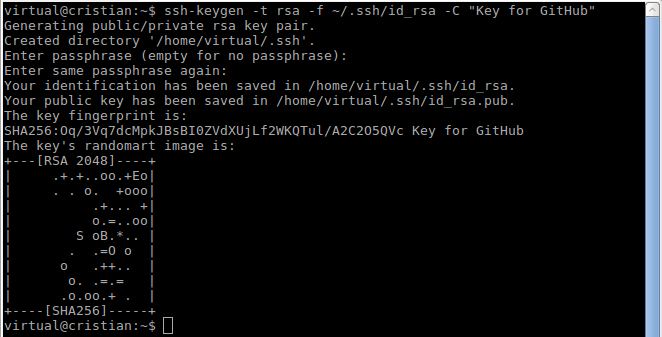
\includegraphics[scale = 0.9]{img/ssh_key.png}
		\caption{Generarea ssh-key}%
		\label{fig:generarea_ssh_key}
	\end{center}
\end{figure}

\begin{figure}[htb]
	\begin{center}
		\centering
		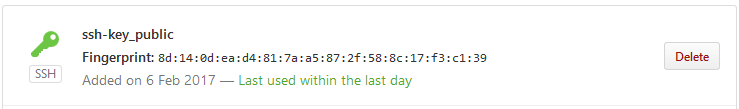
\includegraphics[scale = 0.9]{img/add_key_onserver.png}
		\caption{Adaugarea ssh-key pe server}%
		\label{fig:add_key_onserver}
	\end{center}
\end{figure}

\clearpage